
\documentclass[draftclsnofoot, onecolumn, compsoc, 10pt]{IEEEtran}
\usepackage{lscape}
\usepackage{rotating}
\usepackage{titling}
\usepackage[margin=0.75in]{geometry}
\usepackage{graphicx}
\usepackage{placeins}
\usepackage{caption}
\usepackage{float}
\usepackage{url}
\usepackage{natbib}
\usepackage{setspace}
\usepackage{lscape}
\geometry{textheight=9.5in, textwidth=7in}
\graphicspath{ {images/} }
\linespread{1.0}
\parindent=0.0in
\parskip=0.2in

\title{OS 2 Assignment 2}
\author{Oregon State University\\CS 444\\2018\\\\Prepared By:\\Hayden
Anderson\\Thomas Noelcke\\James Zeng\\}


\def \CapstoneTeamNumber{		41	}
\def \CapstoneProjectName{		Assignment 2 }




\newcommand{\NameSigPair}[1]{\par
\makebox[2.75in][r]{#1} \hfil 	\makebox[3.25in]{\makebox[2.25in]{\hrulefill} \hfill		\makebox[.75in]{\hrulefill}}
\par\vspace{-12pt} \textit{\tiny\noindent
\makebox[2.75in]{} \hfil		\makebox[3.25in]{\makebox[2.25in][r]{Signature} \hfill	\makebox[.75in][r]{Date}}}}

\begin{document}
\begin{titlepage}
    \pagenumbering{gobble}
    \begin{singlespace}
        \hfill
        \par\vspace{.2in}
        \centering
        \scshape{
            \huge OS 2 \par
            {\large\today}\par
            \vspace{1in}
            \textbf{\Huge\CapstoneProjectName}\par
            \vspace{1in}
            {\large Prepared by }\par
            Group\CapstoneTeamNumber\par
            \vspace{5pt}
            \vspace{20pt}
        }
        \vfill
    \end{singlespace}
\end{titlepage}
\newpage
\pagenumbering{arabic}
\clearpage
\tableofcontents
\pagebreak

\section{Algorithm Design}

    The C-Look algorithm is an elevator based algorithm that reads the requests in order from greatest to least. In this section we discuss the position of a hard-drive's write head and how it relates to the center of the disk, where the center of the disk is the lowest position and the outer part is highest. Once the scheduler gets to the lowest request in the queue it will reset the position to the position of the highest request in the queue. Following this algorithm places the write head away from the center of the disk to the point of the highest request. It should be noted that this algorithm is designed to be use with a spinning disk of some kind or another and would not make sense with random access memory.\\

    The C-Look algorithm accomplishes efficient writing by using a circularly linked list where it inserts each request into the list based on the physical position it is requesting. By inserting the items into the circularly linked list in sorted order, we do not need to manually set the position of the drive to the highest position. The circularly linked list works by inserting the items into the list in sorted order and then it naturally wraps around from highest memory address to lowest memory address. Shown below is a visual representation of the position of the write head over time (Fig. 1). \\
\begin{figure}[ht]
\centering
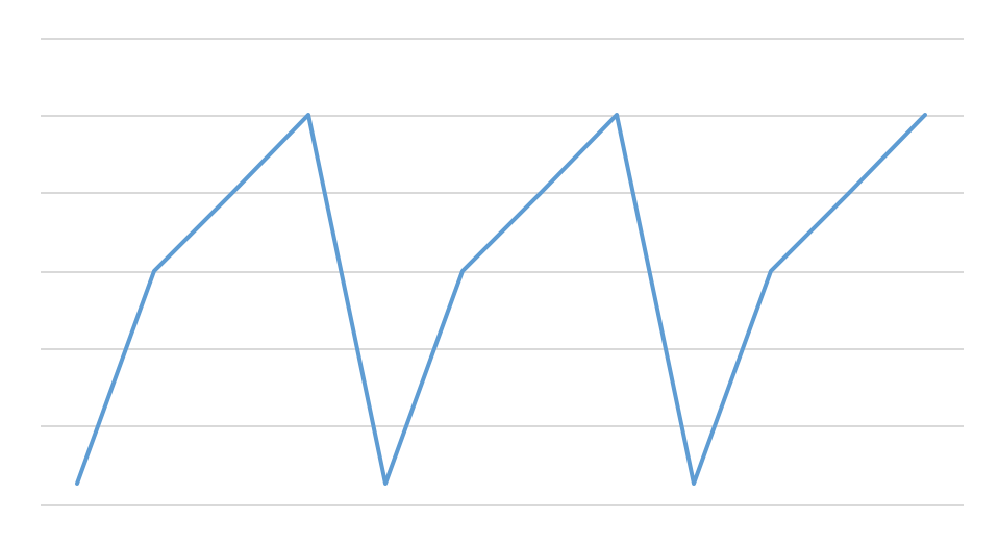
\includegraphics[width=0.3\textwidth]{img.eps}
\caption{\label{fig:graph}This graph shows the location of the disk head with respect to time.}
\end{figure}

\section{Questions}
    \subsection{What do you think the main point of this assignment is?}
    The main point of this assignment was to learn how the Linux kernel implements its I/O scheduling. We had to learn the differences between the different elevators using LOOK and C-LOOK and then decide which one was the best fit for our program.
    \subsection{How did you personally approach the problem? Design Decisions, Algorithm, etc.}
    First, we looked into the source code of the No-op and researched the data structures used to implement this I/O scheduler. Then, we researched the differences between the LOOK and C-LOOK algorithm and how each would be implemented. While researching the No-op file, we noticed that the data structures used to keep track of the requests is a circularly linked list. Due to the use of a circularly linked list, it would be easier to implement C-LOOK instead of LOOK because once the write head reaches the end of the disk head it will automatically point to the beginning of the disk. We looked at the different types of sorts we would need to implement for our version of C-LOOK. We kept the elv\_dispatch\_sort and implemented our own insertion sort in tandem.
    \subsection{How did you ensure your solution was correct? Testing details for instance.}
    To ensure we had the correct solution, we use the printk function to test our program. We print during the dispatch and add\_request function. In the dispatch function, we print whether the kernel dispatches a read request or a write request. We also print the position of the request. The add\_request also prints the position of the request. Now when we run the virtual machine we can see where the head of the requests is located. To ensure that our algorithm works correctly, we can see the location starts at a certain number and then it increases until the head reaches the end of the disk. At this point the head will jump back to the bottom of the disk and the process repeats.
    \subsection{What did you learn?}
    We learned how to implement a LOOK and C-LOOK elevator and the differences between them.
    \subsection{How should the TA evaluate your work? Provide detailed steps to prove correctness}
	The TA should compile our program using make -j4 all. Following the compilation, the TA should use source /scratch/opt/environment-setup-i586-poky-linux. After that they should run the qemu command: qemu-system-i386 -gdb tcp::5541 -S -nographic -kernel arch/x86/boot/bzImage -drive file=core-image-lsb-sdk-qemux86.ext4,if=ide -enable-kvm -net none -usb -localtime --no-reboot --append "root=/dev/hda rw console=ttyS0 debug". After the qemu command, they should run gdb -tui, target remote:5541, continue. Once in the virtual machine they can see that our elevator starts at the head of the disk and once the write head reaches the end it jumps back to the start of the disk. In other words, the elevator only travels in one direction.
	


\newpage

\begin{landscape}

\section{Work Log}
    	\begin{center}
			\begin{tabular}{||c c c c ||}
			\hline
			Name & Task & Date & Total Time\\[0.5ex]
			\hline \hline
			Thomas & Set up document  & 4/24 & 0.5 Hours\\
			\hline
			Thomas, Hayden and James & Started working on C-LOOK scheduler & 4/24 & 2 hours\\
            \hline
            Hayden & Edited what we have so far & 4/25 & 0.5 hours\\
            \hline
            Thomas, James, Hayden & Worked on C-LOOK scheduler & 4/27 & 2 hours\\
            \hline
            Thomas & Worked on configuring and running kernel with new IO scheduler & 5/1 & 3 hours\\
            \hline
            Thomas & Worked on configuration an testing IO scheduler & 5/3 & 1 hour \\
            \hline
            Thomas & Worked on fixing errors that cause faults & 5/3 & 2 hours\\
            \hline
            Thomas & Fixed panic issues and proved that scheduler works & 5/4 & 2 hours\\
            \hline
            James & Finished Report questions & 5/5 & 2 hours\\
            \hline
            Hayden & Read through and edited the paper portion & 5/5 & 1 hours\\
            \hline
            Hayden & Went through report and cleaned up some wording and inconsistencies & 5/5 & 1 hours\\
            \hline
            Thomas & Fixed some styling issues & 5/6 & .25 hours\\
            \hline
            Thomas & Added version control log to the write up and made final revisions & 5/6 & 0.5 hours\\
            \hline
            Thomas & Created Patch file for submission & 5/6 & 1 hour\\
            \hline
			\end{tabular}
		\end{center}
\end{landscape}
\newpage

\section{Version Control Log}
    \begin{verbatim}
commit 334763688f64c67946f48d8cba82b32dce6be754
Author: Thomas Noelcke <noelcket@oregonstate.edu>
Date:   Fri May 4 17:26:14 2018 -0700

    Fixed kernel panic due to scheduler

commit 8960baf090ed906f89dcae5f52aa8fd6fabb735f
Author: Thomas Noelcke <noelcket@oregonstate.edu>
Date:   Thu May 3 23:10:08 2018 -0700

    Trying to get SSTF scheduler to run

commit 4602e012a43f6b78b010383d60f12f19cbd4b43c
Author: Thomas Noelcke <noelcket@oregonstate.edu>
Date:   Tue May 1 22:50:34 2018 -0700

    Worked on setting up config to run scheduler

commit 640762dbd84af0637412c3718ddc15978f092aa2
Author: Thomas Noelcke <noelcket@oregonstate.edu>
Date:   Fri Apr 27 17:13:39 2018 -0700

    worked on sstf scheduler

commit c6da68556c97772c4cb96e868057045d2a2ee778
Author: Hayden Anderson <anderrob@oregonstate.edu>
Date:   Tue Apr 24 17:42:08 2018 -0700

    Started IO Scheduler

\end{verbatim}
\end{document}
